\begin{frame}{Finite Size Analysis of Entanglement Spectra}
\vskip-1.5cm
%\begin{columns}[T]
%\begin{column}{.5\textwidth}
\only<1>{
        \begin{figure}[hbctp]
        \centering
        \includegraphics[width=0.8\textwidth]{{EntanglementEnergyScaling.pdf}}
        %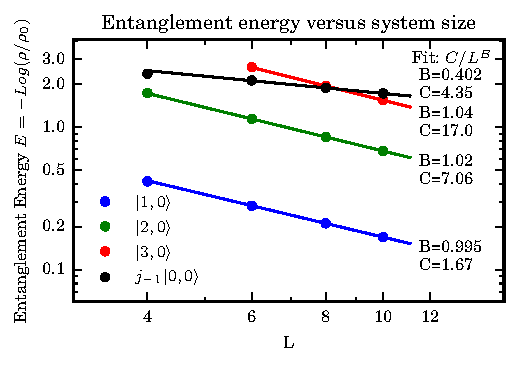
\includegraphics{{interpolatedboson/a10/plots/EntanglementEnergyScaling2.pdf}}
        %\caption{Power law fits for the lowest three states above the ground state at momentum zero and lowest two states at momentum 1 in Figure \ref{fig:sc-EEFinitesize}. The $1/L$ scaling is a signature of a gapless (entanglement) Hamiltonian. The labeling of the states $\ket{e, m}$ or $j_{-1} \ket{e, m}$ is explained in the CFT section below.}
        %\label{fig:sc-EEScaling}
        \end{figure}
%        \bi 
%        \item<1-> Low energy modes show gapless $1/L$ behavior
%        \ei
}
%\end{column}
%\begin{column}{.5\textwidth}
\only<2>{
				\begin{figure}[hbctp]
        \centering
        \includegraphics[width=\textwidth]{{TopologicalEntanglementEntropy.pdf}}
        \end{figure}
}
%\end{column}
%\end{columns}

\end{frame}